\documentclass{article}


\usepackage{arxiv}

\usepackage[utf8]{inputenc} % allow utf-8 input
\usepackage[T1]{fontenc}    % use 8-bit T1 fonts
\usepackage{hyperref}       % hyperlinks
\usepackage{url}            % simple URL typesetting
\usepackage{geometry}
\geometry{margin=0.5in}
\usepackage{multirow}
\usepackage{float}
\usepackage{graphicx}
\usepackage{caption}
\usepackage{filecontents}
\usepackage{subcaption} % Add the subcaption package
\usepackage[title]{appendix}
\usepackage{fancyhdr}
\usepackage{array}
\usepackage{booktabs}       % professional-quality tables
\usepackage{amsfonts}       % blackboard math symbols
\usepackage{nicefrac}       % compact symbols for 1/2, etc.
\usepackage{microtype}      % microtypography
\usepackage{lipsum}
\usepackage{graphicx}
\pagestyle{fancy}
\usepackage{amsmath}
\graphicspath{ {./images/} }
\usepackage[compact]{titlesec}         % you need this package
\titlespacing{\subsection}{0pt}{5pt}{0pt} % this reduces space between (sub)sections to 0pt, for example


\title{COMP 551 Assignment 2 Report - Fall 2024}


\author{
 Hathaway Hao \\
  261071268\\
  %% examples of more authors
   \And
 Yifan Lin \\
  261078741\\
  \And
 Michael Yu \\
  261070826\\
  %% \AND
  %% Coauthor \\
  %% Affiliation \\
  %% Address \\
  %% \texttt{email} \\
  %% \And
  %% Coauthor \\
  %% Affiliation \\
  %% Address \\
  %% \texttt{email} \\
  %% \And
  %% Coauthor \\
  %% Affiliation \\
  %% Address \\
  %% \texttt{email} \\
}

\begin{document}
\maketitle
\begin{abstract}
\textit {This report explores statistical learning techniques applied to synthetic data, focusing on linear regression with non-linear basis functions and regularization methods. We implemented L1 (Lasso) and L2 (Ridge) regularization, performing cross-validation to evaluate model performance under varying regularization strengths. Additionally, we conducted a bias-variance decomposition to access model complexity. The analysis highlights the trade-off between under-fitting and over-fitting, demonstrating the effectiveness of regularization in improving model generalization.}
\end{abstract}

\section{Task 1: Linear Regression with Non-Linear Basis Functions}

\subsection{Introduction}
\noindent The main objective of Task 1 is to explore the effectiveness of Gaussian basis functions in approximating non-linear relationships. We aim to demonstrate how increasing the complexity of a model by adding more basis functions affects its performance, highlighting the trade-off between underfitting and overfitting. Our approach starts with generating synthetic data from a non-linear function, and then attempting to approximate this function using a linear combination of Gaussian basis functions. We then can observe how model complexity by changing the number of basis functions, which influences the quality of fit and generalization performances.


\subsection{Methodology}
\paragraph{Data Generation}
We begin by generating a synthetic dataset that represents a non-linear relationship. The true function is defined as: $y(x) = \sin(\sqrt{x}) + \cos(x) + \sin(x) + \epsilon$, where $x$ is uniformly sampled from the range $[0, 20]$, and $\epsilon$ is Gaussian noise with mean 0 and variance 1. See Figure \ref{data}, the scatter plot of the generated data shows the noisy observations along with the true underlying function. The noise in the data simulates real-world measurement errors, adding complexity to the approximation task.
\begin{figure}[H]
    \centering
    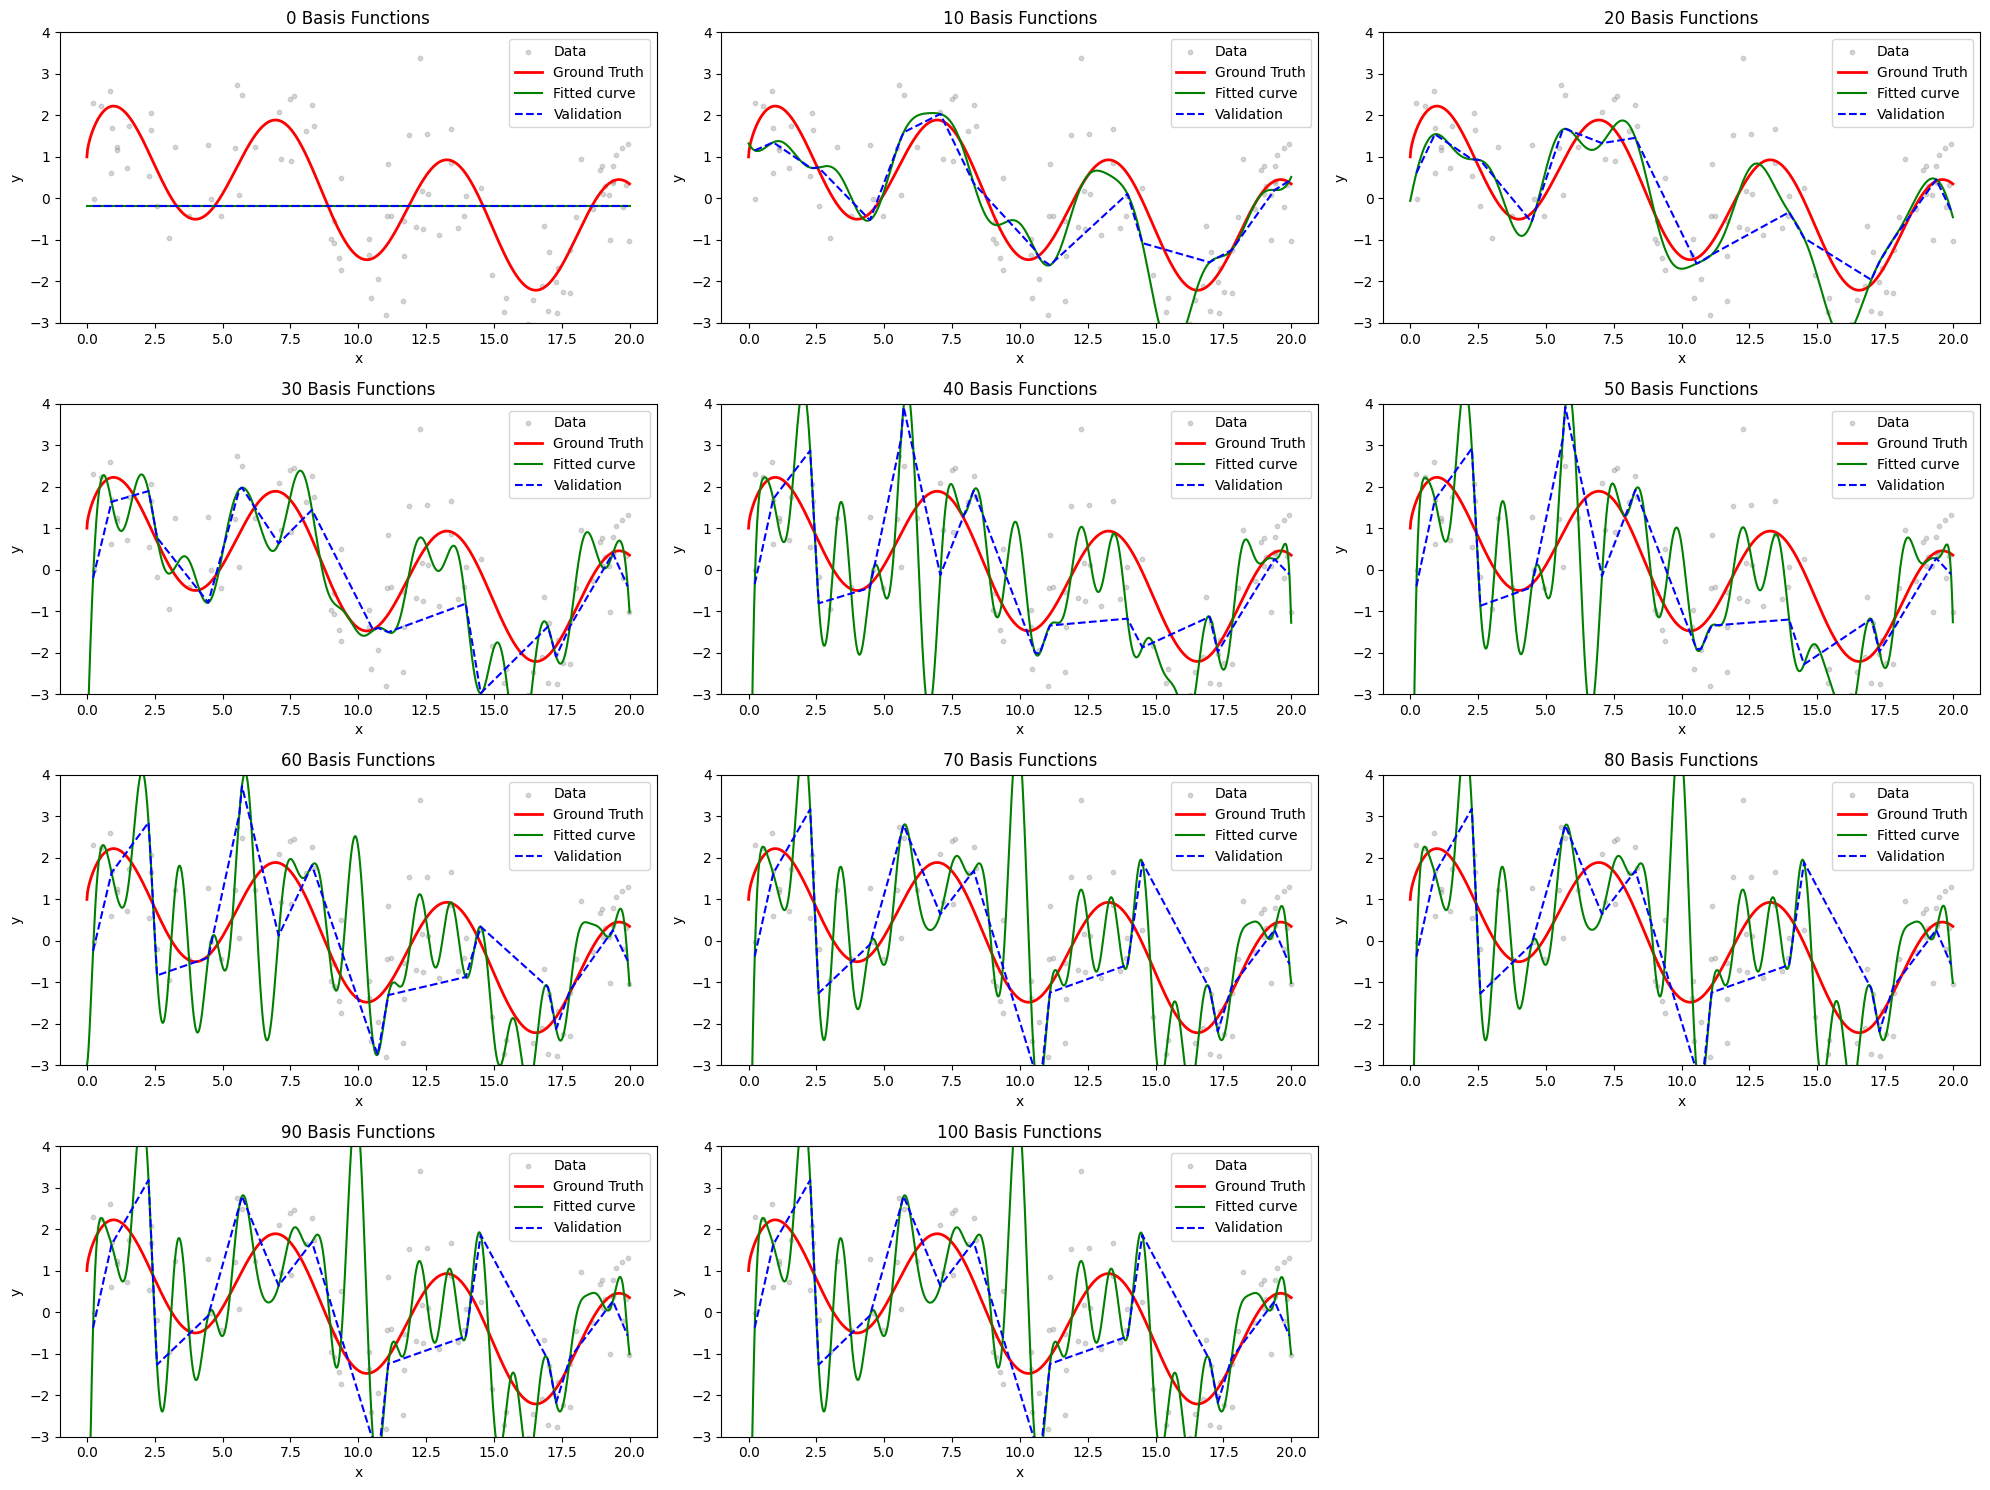
\includegraphics[width=1\linewidth,height=0.26\textheight]{figures/gaussian_data.png} 
    \caption{LinearRegression model fitting with Gaussian function at the range for 0,10,20, ..., 100}
    \label{gaussian data}
\end{figure}

\paragraph{Gaussian Basis Functions}
To explore the Gaussian basis function, we transform the original input features by using Gaussian basis functions of the form:
$\varphi(x, \mu, \sigma) = \exp\left(-\frac{(x - \mu)^2}{2\sigma^2}\right)$
Where $\mu$ is the mean of the Gaussian and $\sigma$ is the standard deviation. We fix $\sigma = 1$ and vary the number of basis functions from 0 to 100, with their centers ($\mu$) evenly spaced across the input range. Shown in Figure \ref{gaussian}, demonstrates how these functions can capture local patterns in the data. Each basis function responds to inputs near its center and to distant inputs.

\paragraph{Model Fitting}
We split the data to train and validation sets and implemented a linear regression class that fits the model using the pseudoinverse method with train data. Here, we can visualize the fitted curves with training sets and validation sets alongside the true function and the noisy data points after fitting multiple models, shown in Figure \ref{gaussian data}, each with a different number of basis functions (0, 10, 20, ..., 100).
\begin{figure}[H]
    \centering
    \begin{minipage}{0.45\textwidth}
        \centering
        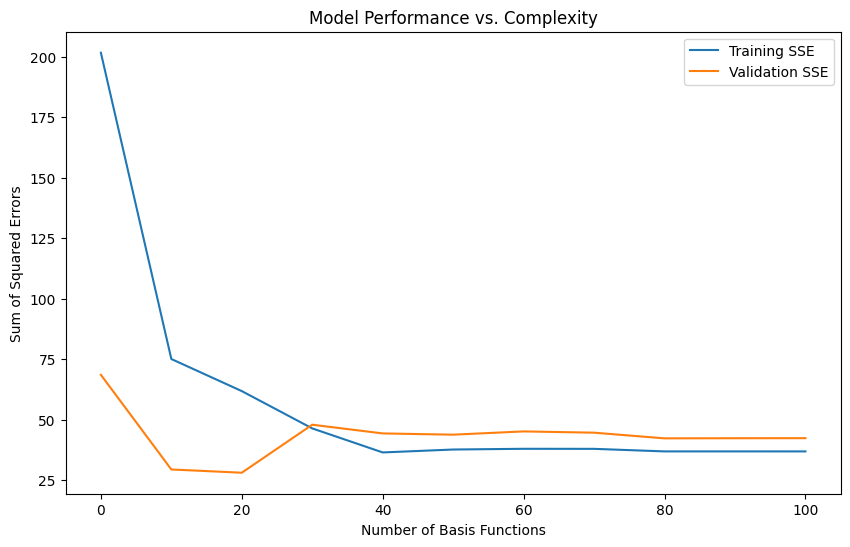
\includegraphics[width=\linewidth, height=0.45\linewidth]{figures/complexity.png} 
        \caption{SSE for fitted models in range of Gaussian basis}
        \label{SSE}
    \end{minipage}
    \centering
    \begin{minipage}{0.50\textwidth}
        \centering
        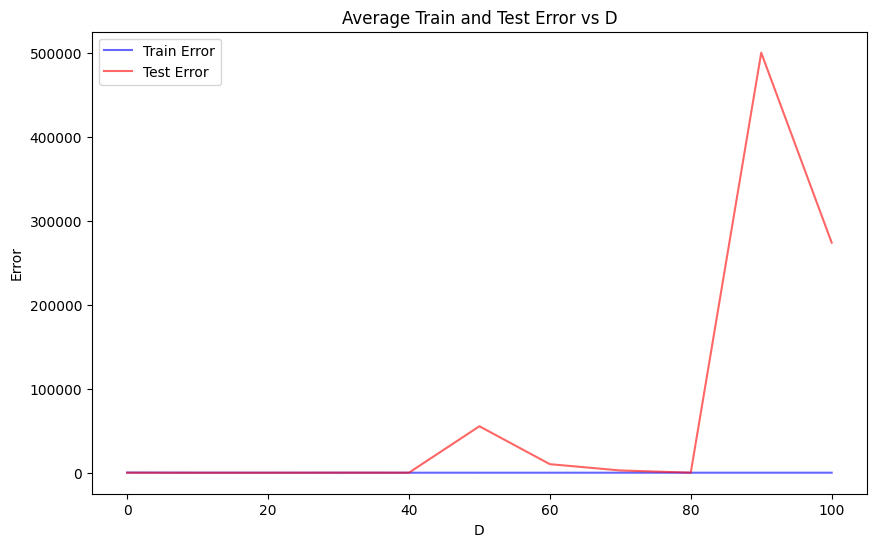
\includegraphics[width=\linewidth, height=0.45\linewidth]{figures/average_error.png} 
        \caption{Bias-Variance Trade-off}
        \label{error_compare}
    \end{minipage}
\end{figure}

\paragraph{Model Selection}
To select optimal model complexity, we again split the data into training and validation sets. Then we compute the Sum of Squared Errors (SSE) for each model on both sets. See Figure \ref{SSE} and Table \ref{SSE_table}, the results show a clear pattern of model performance across different numbers of Gaussian basis functions. With 0 basis functions, both training and validation SSE are high. As the number of basis functions increases, we observe a rapid decrease in both training and validation SSE. The optimal model complexity is achieved with 20 basis functions, where the validation SSE reaches its minimum of 28.14.


\subsection{Conclusion and Discussion}
By plotting SSE on both sets, we observed that 20 Gaussian basis functions provide the optimal balance between fitting the data and generalizing to unseen points. Models with fewer basis functions (0-10) showed clear underfitting, with high SSE values for both training and validation sets. Conversely, models with more than 20 basis functions exhibited overfitting, with decreasing training SSE but increasing validation SSE. Also, it is worth mentioning that model performance stabilized for very high numbers of basis functions (80-100), suggesting inherent regularization in our approach. Interestingly, this task demonstrates that very complex models may not perform much worse than moderately complex ones in some cases, possibly due to implicit regularization in the fitting procedure. It is important to note that input transformations can enable simple models to capture complex relationships (Myung et al., 2000)\ref{model_complexity}, and they can provide a clear illustration of the bias-variance trades-off.


\section{Task 2: Bias-Variance Tradeoff with Multiple Fits}

\subsection{Introduction}
In Task 2, we aim to understand the balance between a model's ability to capture bias and variance, which is crucial for building effective predictive models. This task explores the bias-variance trade-off in the context of non-linear function approximation using Gaussian basis functions.

\subsection{Methodology}
we extend our exploration of Gaussian basis function regression by repeating the process 10 times with resampled data. For each iteration, we generate 100 new data points from the same non-linear function as Task 1 data generation. We then fit linear regression models using Gaussian basis functions with different ranges as well.

\begin{figure}[H]
    \centering
    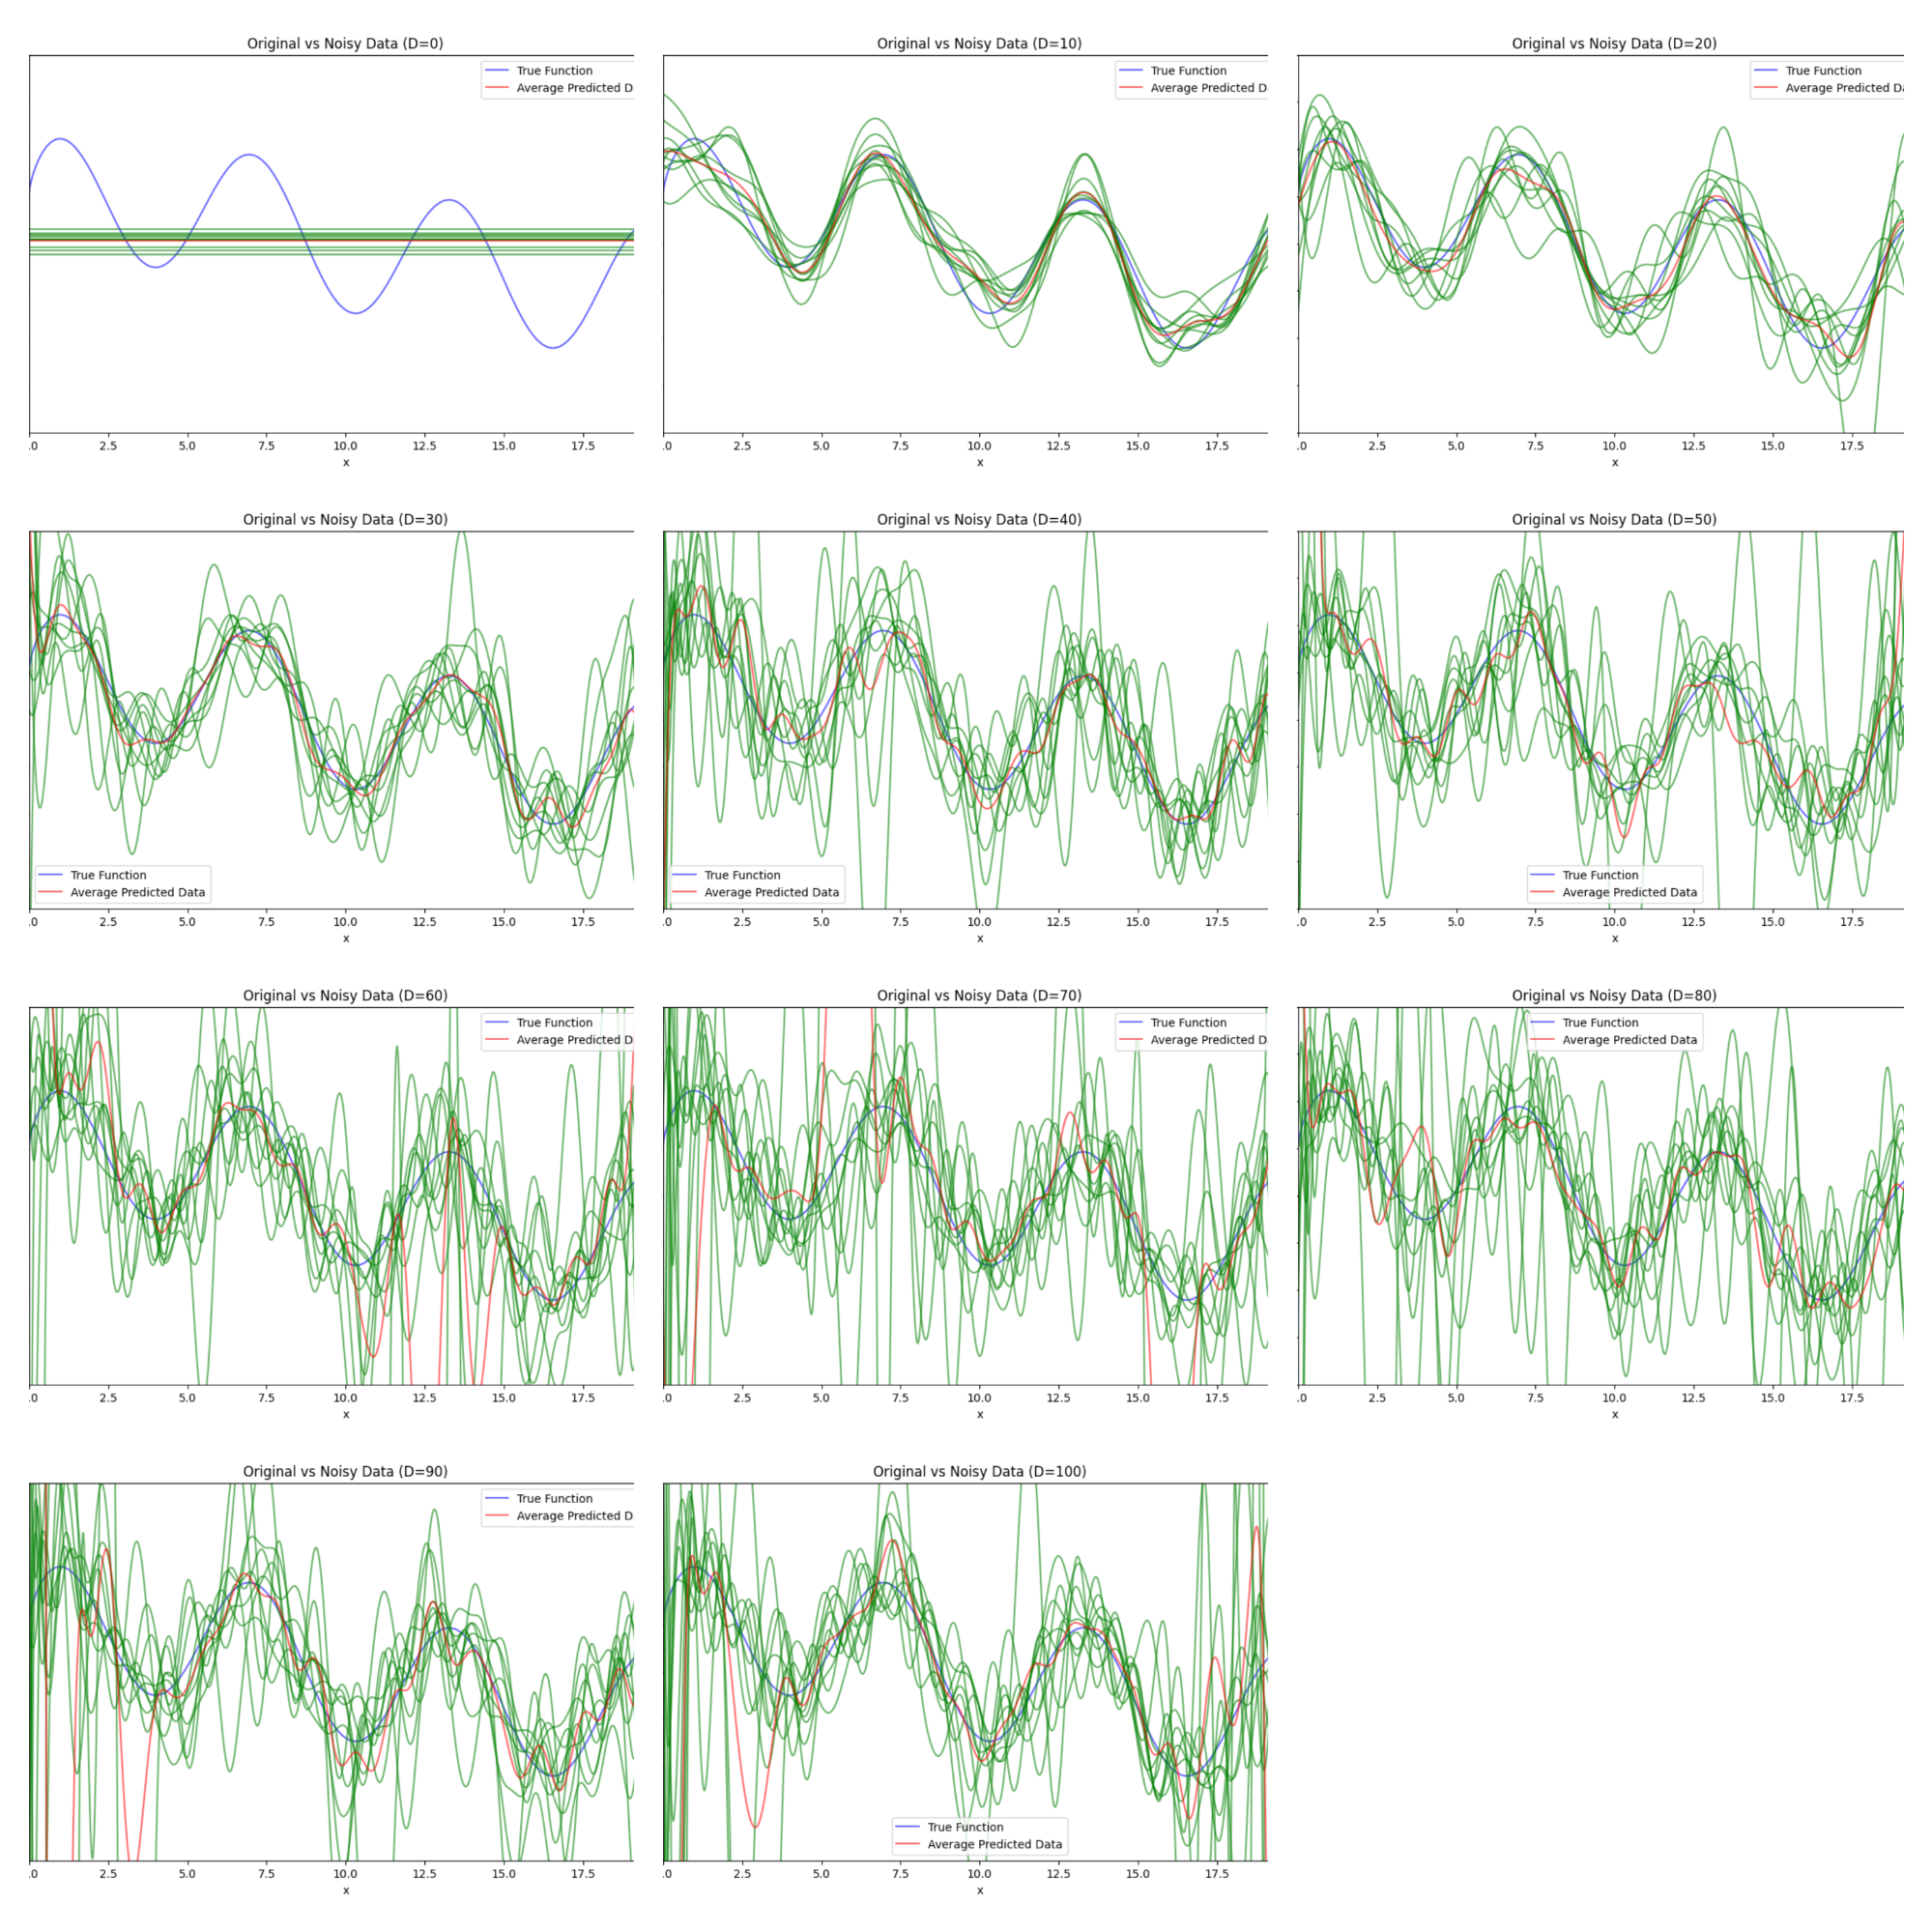
\includegraphics[width=1\linewidth,height=0.3\textheight]{figures/bias_variance.jpg} 
    \caption{Bias-Variance Trade-off}
    \label{bias_variance}
\end{figure}

As Figure \ref{bias_variance} illustrated, the true underlying function (blue line), and the average of the 11 fitted models (red line) on the same graph. This visualization is created for each level of model complexity. Additionally, we compute and plot the average training and test errors across the 11 iterations for each level of complexity. Also, the model result of the average error is shown in Figure \ref{error_compare}, the plots provide a clear visualization of the bias-variance trade-off as the model complexity increases. 

\subsection{Conclusion}
The error plots and bias-variance trade-off visualizations give a clear picture of the model's behavior. For few basis functions (D=0-10), there's high bias and low variance, meaning the model underfits the data. In the range of 20-40, the model balances bias and variance, capturing the true pattern well. However, beyond 60 basis functions, both the error plot and bias-variance graph show overfitting, with a sharp rise in test error. The ideal model, achieving the best balance, uses around 30 basis functions.

\section{Task 3: Regularization with Cross-Validation}

\subsection{Introduction}
\noindent Introduction
In this task, we implemented both \textbf{L1 (Lasso)} and \textbf{L2 (Ridge)} regularization in a linear regression model using synthetic data transformed by Gaussian basis functions. We evaluated model performance via cross-validation with regularization parameter $\lambda$ values from $10^{-4}$ to $10^2$ and performed a \textbf{bias-variance decomposition} to assess the impact of regularization on model complexity. The following details the implementation and analyzes the resulting error and bias-variance graphs.


\subsection{Methodology}

\paragraph{Implementation of L1 and L2 Regularization}
For \textbf{L1 (Lasso)}, the goal is to minimize the sum of squared residuals while penalizing the absolute values of the weights, with the loss function:
$J(w) = \frac{1}{2m} \sum_{i=1}^{m} \left( y^{(i)} - w^T x^{(i)} \right)^2 + \lambda \sum_{j=1}^{n} \left| w_j \right|$
A larger $\lambda$ forces more weights to zero, creating a sparser model.

For \textbf{L2 (Ridge)}, the penalty applies to the squared weights, leading to:
$J(w)=\frac{1}{2 m} \sum_{i=1}^m\left(y^{(i)}-w^T x^{(i)}\right)^2+\frac{\lambda}{2} \sum_{j=1}^n w_j^2$
This shrinks weights without forcing them to zero, with $\lambda$ controlling regularization strength.

Both regularization methods were implemented by adjusting the loss functions and using gradient descent for weight updates.

\paragraph{Cross-Validation for Model Assessment}
We employed \textbf{10-fold cross-validation} for each $\lambda$ value, computing training and validation \textbf{MSE} as:
$\mathrm{MSE}=\frac{1}{m} \sum_{i=1}^m\left(y^{(i)}-\hat{y}^{(i)}\right)^2$
Averaging the MSE across folds provided a reliable estimate of model generalization.

\paragraph{Bias-Variance Decomposition}
The bias squared was calculated as:
$\operatorname{Bias}^2=\frac{1}{m} \sum_{i=1}^m\left(\mathbb{E}\left[\hat{y}^{(i)}\right]-y^{(i)}\right)^2$

Variance measured prediction variability across datasets:
$\text{Variance}=\frac{1}{m} \sum_{i=1}^m \mathbb{E}\left[\left(\hat{y}^{(i)}-\mathbb{E}\left[\hat{y}^{(i)}\right]\right)^2\right]$

The total error was the sum of bias squared, variance, and noise variance.

\begin{itemize} \item \textbf{L2 regularization}: $\lambda$ increased, bias increased, variance decreased, total error rose due to oversimplification. \item \textbf{L1 regularization}: Bias increased, but variance was more stable, retaining some flexibility compared to L2. \end{itemize}

\paragraph{Selection of Optimal $\lambda$}
The optimal $\lambda$ was chosen where validation error was minimized, around $\lambda \approx 10$ for both regularization types. This balance between bias and variance was further supported by the bias-variance decomposition, minimizing total error.

\subsection{Conclusion}
\begin{figure}[h]
    \centering
    \begin{minipage}{0.50\textwidth}
        \centering
        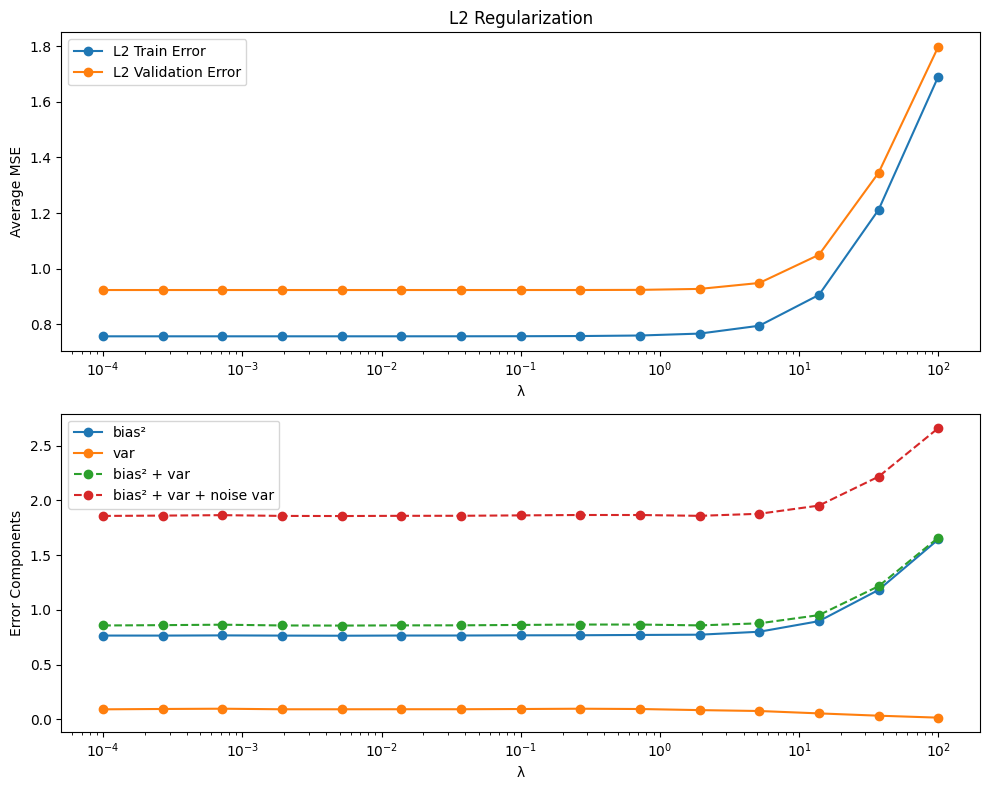
\includegraphics[width=\textwidth]{figures/L2_Regularization.png} 
        \caption{L2 Regularization}
        \label{L2}
    \end{minipage}\hfill
    \begin{minipage}{0.50\textwidth}
        \centering
        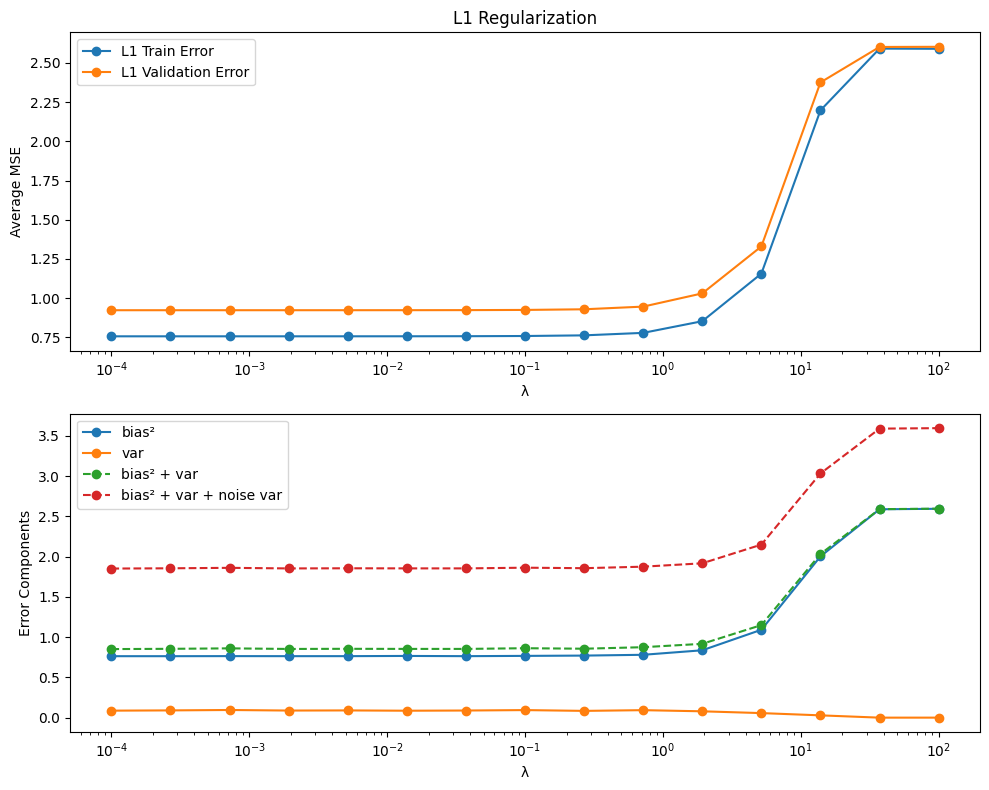
\includegraphics[width=\textwidth]{figures/L1_Regularization.png} 
        \caption{L1 Regularization}
        \label{L1}
    \end{minipage}
\end{figure}

For small $\lambda$, both L1 and L2 regularization resulted in low training errors but high validation errors, shows overfitting. As $\lambda$ increased, training errors rose while validation errors initially decreased, then increased at large $\lambda$, shows underfitting.

The bias-variance decomposition confirmed this: $\bullet$ Small $\lambda$ led to high variance and low bias, causing overfitting. $\bullet$ Increasing $\lambda$ raised bias and lowered variance, minimizing error at an intermediate $\lambda$.

The optimal $\lambda$ was selected where validation and total errors were minimized, balancing bias and variance. Overall, L1 and L2 regularization reducing overfitting at small $\lambda$ and underfitting at large $\lambda$. Cross-validation reliably identified the optimal $\lambda$ as shown.


\section{Task 4: Effect of L1 and L2 Regularization on Loss}

\subsection{Introduction}
\noindent This task examines the effects of \textbf{L1 (Lasso)} and \textbf{L2 (Ridge)} regularization on linear regression models using synthetic data. We investigate regularization strengths ($\lambda$) ranging from 0.01 to 10. The analysis involves visualizing loss function contours and gradient descent paths for each regularization type and strength. This approach allows for a comparative assessment of how L1 and L2 regularization influences the optimization landscape and convergence behavior in linear regression problems. The findings provide insights into the characteristics and impacts of these regularization techniques on model fitting and parameter estimation.

\subsection{Methodology}
\noindent We compare L1 and L2 regularization using four regularization strengths ($\lambda$): 0.01, 0.1, 1, and 10. For each combination, we visualize the optimization landscape through loss function contours and overlay gradient descent paths to show the optimization trajectory.

\subsection{Conclusion}
\begin{figure}[h]
    \centering
    \begin{minipage}{1\textwidth}
        \centering
        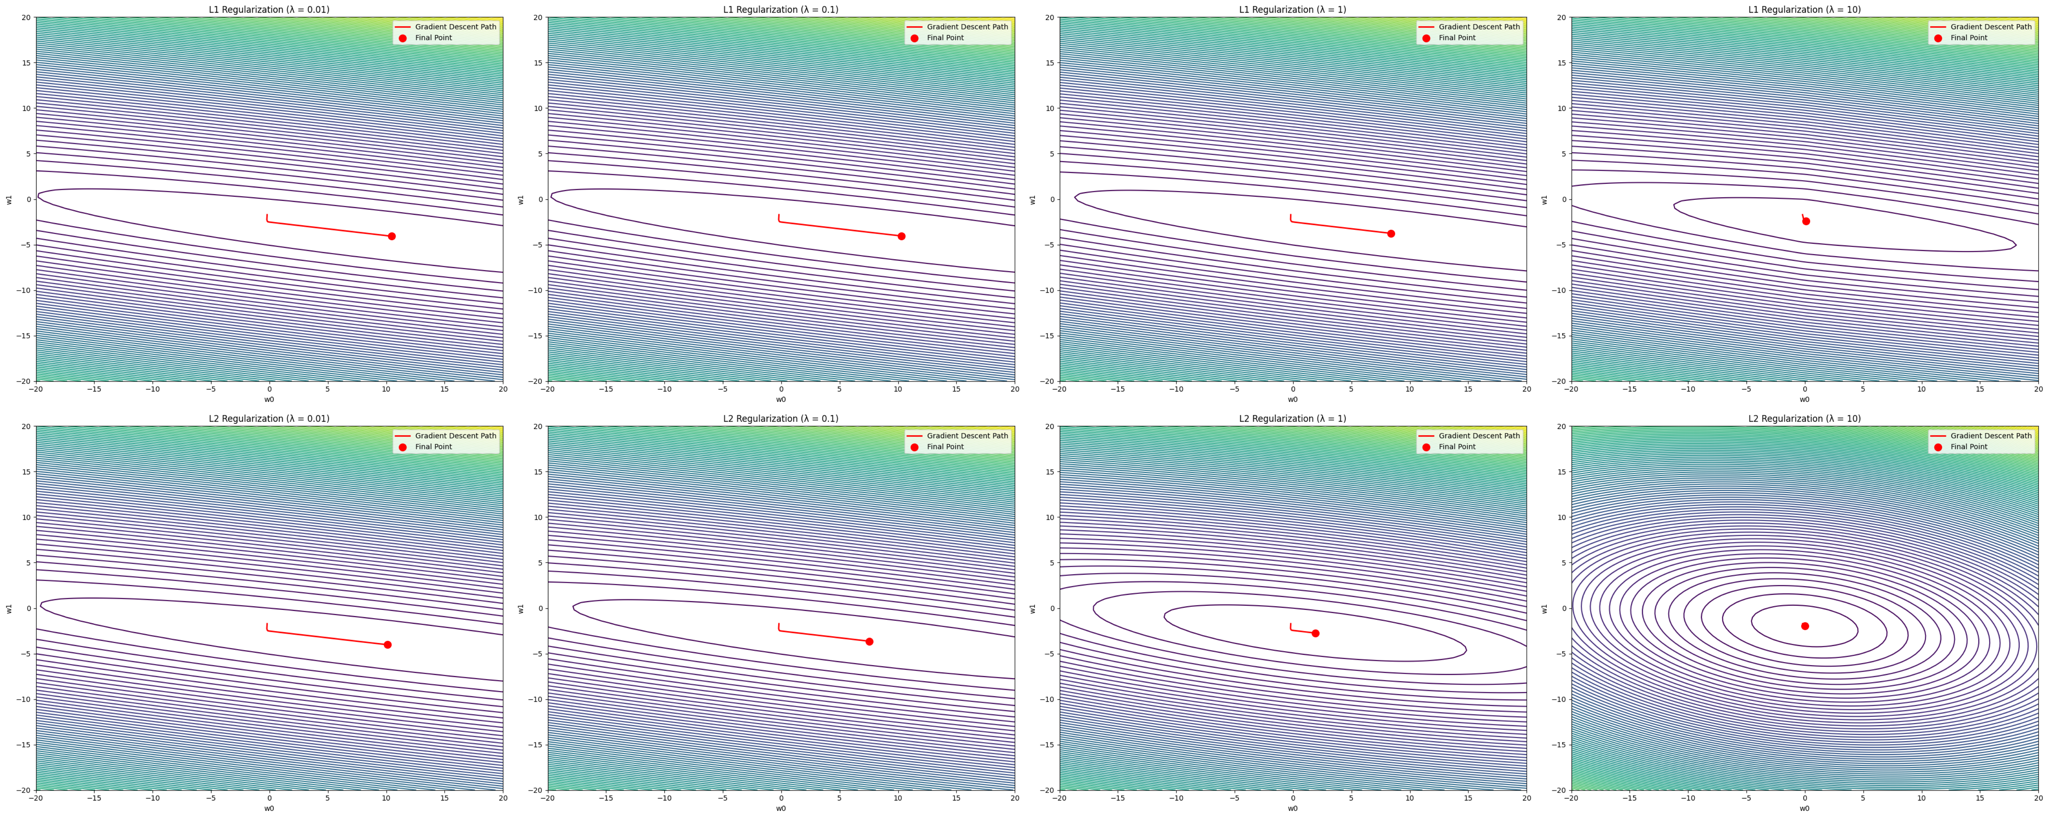
\includegraphics[width=\textwidth]{figures/T4.png} 
        \caption{L1 and L2 Regularization ($\lambda$ = 0.01, 0.1, 1, 10)}
    \end{minipage}
\end{figure}

L1 regularization encourages sparsity by driving some weights to exactly zero. This is evident in the plots, especially for higher $\lambda$ values (1 and 10), where the optimization paths move towards the axes. The final points for $\lambda = 10$ in L1 regularization are very close to one axis, indicating that one weight is nearly zero. The diamond-shaped contours of the loss landscape, particularly pronounced at higher $\lambda$ values, further illustrate this sparsity-inducing property.

L2 regularization typically penalizes large weights but does not promote sparsity as strongly as L1. For lower $\lambda$ values, both L1 and L2 show similar behavior. At higher $\lambda$ values, particularly $\lambda$=10, the L2 plot shows more circular contours, indicating uniform penalization in all directions.

As $\lambda$ increases from 0.01 to 10, both regularization types show stronger effects:\\
For L1: The paths become shorter and more curved, moving along or towards the axes. The loss landscape contours become more diamond-shaped, emphasizing the sparsity-inducing effect.\\
For L2: The paths also shorten but remain more direct. The loss landscape contours become more circular, illustrating the uniform penalization of weights.

\section{Discussion and Conclusion}

Found that 20 Gaussian basis functions provided the optimal balance between underfitting and overfitting. Notably, models showed unexpected stability at higher numbers (80-100), suggesting inherent regularization in the approach.

Demonstrated clear patterns where low basis functions (0-10) showed high bias and low variance, optimal performance at 20-40 bases, and severe overfitting beyond 60 bases. The analysis provided visual confirmation through error plots and bias-variance trade-off visualizations.

Both L1 and L2 regularization effectively controlled model complexity. Small $\lambda$ led to overfitting (high variance, low bias), while increasing $\lambda$ raised bias and lowered variance. Cross-validation successfully identified the optimal $\lambda$ that minimized validation error.

Compared L1 and L2 regularization effects through loss landscape visualization. L1 showed clear sparsity-inducing properties with diamond-shaped contours and paths moving toward axes, while L2 demonstrated more uniform weight penalization with circular contours. Higher $\lambda$ values amplified these distinctive characteristics.

\section{Statement of Contributions}

All members contributed equally to this project. We each completed the lab independently and then combined our individual work and code to produce the final report.

\newpage
\bibliographystyle{unsrt}  
%\bibliography{references}  %%% Remove comment to use the external .bib file (using bibtex).
%%% and comment out the ``thebibliography'' section.

%%% Comment out this section when you \bibliography{references} is enabled.
\begin{thebibliography}{1}

\bibitem{model complexity} Myung, I. J. (2000). The importance of complexity in model selection. Journal of mathematical psychology, 44(1), 190-204.
\label{model_complexity}

\bibitem{Lecture notes} Prémont-Schwarz, I. (2023). Gradient Descent. COMP 551, McGill University.\label{ref:lectures}


\end{thebibliography}

\begin{appendices}


\section{Task 1}

\subsection{Data Generation and Gaussian Basis Function} \label{app:loss-history-sgd}

\begin{figure}[h]
    \centering
    \begin{minipage}{0.45\textwidth}
        \centering
        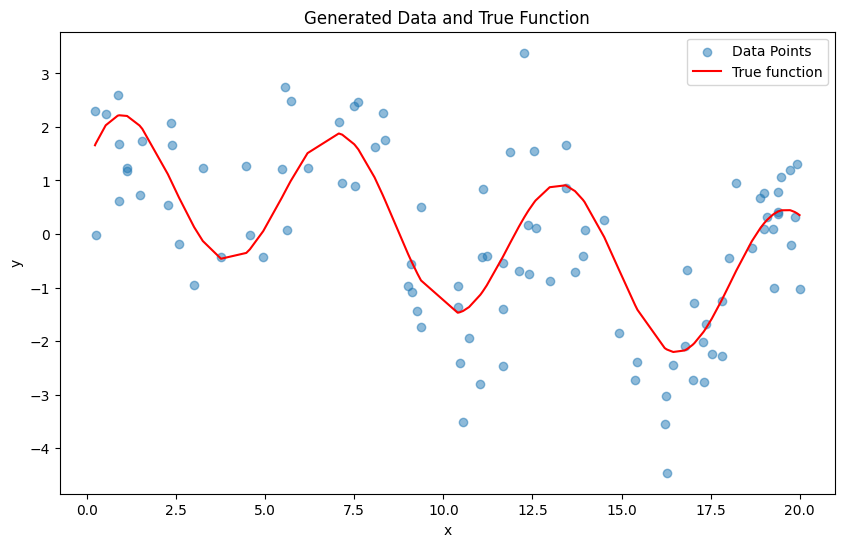
\includegraphics[width=\textwidth]{figures/data.png} 
        \caption{Non-linear data generation}
        \label{data}
    \end{minipage}\hfill
    \begin{minipage}{0.55\textwidth}
        \centering
        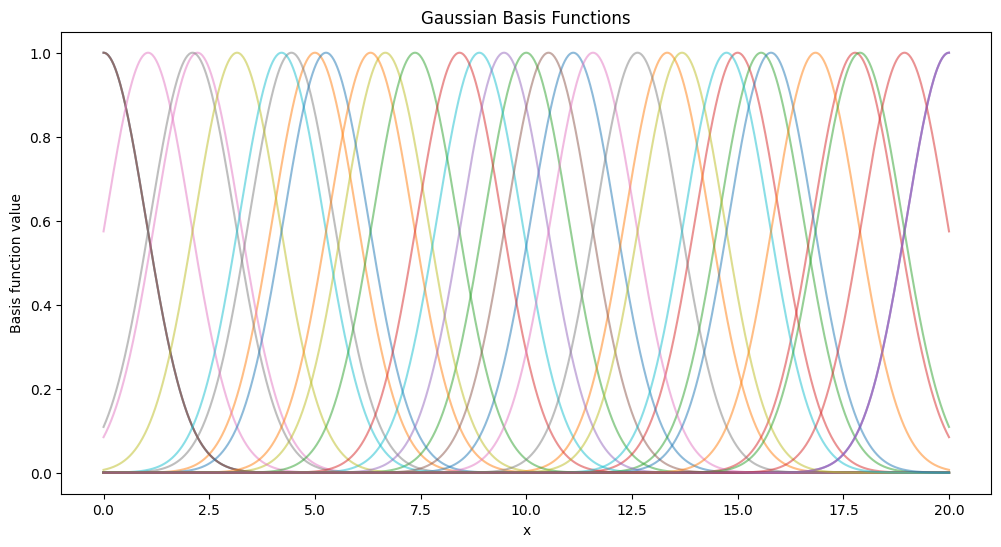
\includegraphics[width=\textwidth]{figures/gaussian_basis.png} 
        \caption{Gaussian basis for range of generated data}
        \label{gaussian}
    \end{minipage}
\end{figure}

\subsection{SSE for Fitted models in the Range of Gaussian
basis} \label{app:loss-history-sgd-log}
\begin{minipage}{0.5\textwidth}  % Adjust width as needed
        \centering
        \begin{tabular}{|c|c|c|}
            \hline
            {Number of Bases} & {Training SSE} & {Validation SSE} \\
            \hline
             0  & 201.64  & 68.58  \\
            10  &  75.11  & 29.48  \\
            20  &  61.85  & 28.14  \\
            30  &  46.44  & 47.97  \\
            40  &  36.52  & 44.37  \\
            50  &  37.72  & 43.86  \\
            60  &  38.02  & 45.20  \\
            70  &  38.00  & 44.68  \\
            80  &  36.94  & 42.33  \\
            90  &  36.95  & 42.39  \\
           100  &  36.94  & 42.41  \\
            \hline
        \end{tabular}\\
        \vspace{0.3cm}
        \textbf{Optimal number of basis functions: 20}
        \captionof{table}{Training and validation SSE }
        \label{SSE_table}
    \end{minipage}


\end{appendices}

\end{document}

